\documentclass{beamer}
\usepackage{graphicx}

\let\epsilon\varepsilon
\newcommand{\Mon}{\operatorname{Mon}\;}
\newcommand{\Inv}{\operatorname{Inv}\;}
\newcommand{\pskip}{\medskip}

\title{One-relation semigroups and their word problem}
\author{Lucas Jones}
\date{3rd April, 2017}
\institute{University of St Andrews}

\beamertemplatenavigationsymbolsempty
\definecolor{inactive}{RGB}{230,230,230}

\begin{document}

\maketitle

\begin{frame}{Groups, semigroups, monoids}
	A \textbf{\textcolor{inactive}{semi}group} is a set $S$ together with a binary operation $\cdot \colon S \times S \to S$ such that:

	\begin{enumerate}
		\item \emph{[Associativity]} $(a \cdot b) \cdot c = a \cdot (b \cdot c)$ for all $a, b, c \in S$
		\item \emph{[Identity]} there exists a distinguished element $\epsilon \in S$ such that $\epsilon \cdot x = x \cdot \epsilon = x$ for all $x \in S$
		\item \emph{[Inverses]} for every element $x \in S$, there exists a unique element $x^{-1} \in S$ such that $x \cdot x^{-1} = x^{-1} \cdot x = \epsilon$
	\end{enumerate}
\end{frame}

\begin{frame}{Groups, semigroups, monoids}
	A \textbf{semigroup} is a set $S$ together with a binary operation $\cdot \colon S \times S \to S$ such that:

	\begin{enumerate}
		\item \emph{[Associativity]} $(a \cdot b) \cdot c = a \cdot (b \cdot c)$ for all $a, b, c \in S$
		\textcolor{inactive}{
		\item \emph{[Identity]} there exists a distinguished element $\epsilon \in S$ such that $\epsilon \cdot x = x \cdot \epsilon = x$ for all $x \in S$
		\item \emph{[Inverses]} for every element $x \in S$, there exists a unique element $x^{-1} \in S$ such that $x \cdot x^{-1} = x^{-1} \cdot x = \epsilon$
			}
	\end{enumerate}
\end{frame}

\begin{frame}{Groups, semigroups, monoids}
	A \textbf{monoid} is a set $S$ together with a binary operation $\cdot \colon S \times S \to S$ such that:

	\begin{enumerate}
		\item \emph{[Associativity]} $(a \cdot b) \cdot c = a \cdot (b \cdot c)$ for all $a, b, c \in S$
		\item \emph{[Identity]} there exists a distinguished element $\epsilon \in S$ such that $\epsilon \cdot x = x \cdot \epsilon = x$ for all $x \in S$
		\textcolor{inactive}{
		\item \emph{[Inverses]} for every element $x \in S$, there exists a unique element $x^{-1} \in S$ such that $x \cdot x^{-1} = x^{-1} \cdot x = \epsilon$
			}
	\end{enumerate}
\end{frame}


\begin{frame}{Free semigroups}
	Let $A$ be a finite set.

	Then the \textbf{free semigroup} on $A$, denoted $A^+$, is the set of all words with letters in $A$, under the operation of concatenation. \phantom{, \emph{including an empty string $\epsilon$}}

	\pause
	\bigskip

	\begin{block}{Example}
		If $A = \{a, b\}$, then $A^+ = \{a, b, aa, ab, ba, bb, aaa, aab, \ldots\}$. \\
		Multiplying, $aa \cdot b = aab$.
	\end{block}
\end{frame}

\begin{frame}{Free monoids}
	Let $A$ be a finite set.

	Then the \textbf{free monoid} on $A$, denoted $A^*$, is the set of all words with letters in $A$, under the operation of concatenation, \emph{including an empty string $\epsilon$}.

	\bigskip

	\begin{block}{Example}
		If $A = \{a, b\}$, then $A^* = \{\epsilon, a, b, aa, ab, ba, bb, aaa, aab, \ldots\}$. \\
		Multiplying, $ba \cdot \epsilon = ba$.
	\end{block}
\end{frame}

\begin{frame}{Presentations}
	In the free semigroup and the free monoid, elements don't interact with each other --- \textbf{except} when they are forced to by the axioms.\pskip

	\pause
	A succinct way of describing a semigroup is by a \textbf{presentation}. We start with a free semigroup and add in `relations' describing how the elements interact.

\end{frame}

\begin{frame}{Semigroup presentations}
	(Finite) presentations take the form:
	\[
		\langle \; \overbrace{a_1, a_2, \ldots, a_m}^{\text{generators}}
			\mid 
			\underbrace{u_1 = v_1, \ldots, u_n = v_n}_{\text{relations}} \;
			\rangle
	\]
	Here, $a_1, \ldots, a_n$ are letters in an alphabet $A$, and the $u_i$, $v_i$ are words in $A^+$.\pskip

	The semigroup given by a presentation is the `biggest' or `most general' semigroup which satisfies all of the relations.
\end{frame}

\begin{frame}{Semigroup presentations}
	Some examples:
	\pause
	\begin{itemize}
		\item
			The cyclic group of order 7 $C_7$ is presented by $\langle a \mid a^8 = a\rangle$.\medskip

			The elements are $\{a\}^+ = \{a, aa, aaa, \ldots\}$ --- except that $a^8 = a$, hence $a^9 = a^2$, and so on. So $C_7 = \{a, a^2, \ldots, a^7\}$.\bigskip
		
		\pause
		\item
			The free semigroup on two letters is presented by $\langle a, b \mid \rangle$.\medskip

			The elements are just $\{a, b\}^+$, and there are no more equations that hold.
	\end{itemize}
\end{frame}

\begin{frame}{Monoid presentations}
	Monoid presentations are just like semigroup presentations...
	\[
		\Mon \langle \; \overbrace{a_1, a_2, \ldots, a_m}^{\text{generators}}
			\mid 
			\underbrace{u_1 = v_1, \ldots, u_n = v_n}_{\text{relations}} \;
			\rangle
	\]
	except we start with the free \emph{monoid}, so we have an identity (the empty string $\epsilon$). The words $u_i$ and $v_i$ are in the free monoid $A^*$.
\end{frame}

\begin{frame}{Monoid presentations}
	We can equally define every monoid presentation
	\[
		\Mon \langle a_1, a_2, \ldots, a_m
			\mid 
			u_1 = v_1, \ldots, u_n = v_n
			\rangle
	\]
	in terms of a semigroup presentation
	\begin{align*}
		\langle \epsilon, a_1, \ldots, a_m
		\mid&
		u_1 = v_1, \ldots, u_n = v_n, \\
		& a_1\epsilon = \epsilon a_1 = a_1,
		\ldots,
		a_m\epsilon = \epsilon a_m = a_m
		\rangle.
	\end{align*}
\end{frame}

\begin{frame}{Monoid presentations}
	Some examples:
	\pause
	\begin{itemize}
		\item
			The group of integers under addition has the monoid presentation
				\[ \Mon \langle a, \bar a \mid a\bar a = \bar a a = \epsilon \rangle. \]
			Here $a$ corresponds to 1; $\bar a$ corresponds to -1 and $\epsilon$ corresponds to $0$.
		\bigskip
		\pause
		\item
			The bicyclic monoid is presented by \[ \Mon \langle b, c \mid bc = \epsilon \rangle. \]
			This monoid has elements of the form $c^i {b\,}^j$ for $i, j \in \mathbb{N}_0$.
	\end{itemize}
\end{frame}

\begin{frame}{The word problem}
	An algorithmic problem first considered by Dehn (1911) and Thue (1914).\pskip

	Suppose
		\[ \langle a_1, \ldots, a_m \mid u_1 = v_1, \ldots, u_n = v_n \rangle \]
	is a finite presentation for a (semi)group or monoid.\medskip
	
	Then the \textbf{word problem} asks: given two words $a$ and $b$ in the free (semi)group or monoid, do $a$ and $b$ represent the same element in the (semi)group or monoid given by the presentation?\pskip

	That is, can we get from the word $a$ to the word $b$ just by using the equations in the presentation?
\end{frame}

\begin{frame}{The word problem}
	Suppose we have a free monoid $\Mon \langle a_1, \ldots, a_m \mid\rangle$.\pskip

	Then given two words $u$ and $v$ in $\{a_1, \ldots, a_m\}^*_,$ we have no equations in our presentation. So they only represent the same element if they are equal letter by letter.\pskip

	e.g. in $\Mon\langle a, b \mid\rangle$, $abbabab = abbabab$, but $abbabab \ne bab$, or any other word for that matter...
\end{frame}

\begin{frame}{The word problem}
	Consider the bicyclic monoid \[ B = \Mon \langle b, c \mid bc = \epsilon \rangle. \]

	If we have two words $u, v \in \{b, c\}^*$, then we can go through them both removing $bc$ whenever we see it. This gives us words of the form $c^i {b\;}^j$ ($i, j \in \mathbb{N}_0$) --- $u$ and $v$ represent the same element in $B$ if and only if the indices of $c$ and $b$ are the same in both words.

	% Confuent, noetherian rewriting system?
\end{frame}

\begin{frame}{General monoids and (semi)groups}
	What about the word problem for any monoid presentation? Or any (semi)group presentation?\pskip

	\pause
	Post (1947) showed that there is no algorithm that will solve the word problem for any given presentation.\pskip

	But we can for some. What are the sufficient conditions for the word problem to be solvable?
\end{frame}

\begin{frame}{One-relation (semi)groups and monoids}
	A (semi)group or monoid is \textbf{one-relation} if it is given by a presentation of the form
		\[ \langle a_1, a_2, \ldots \mid u = v \rangle, \]
	i.e. a presentation with one relation.\pskip

	\pause
	\begin{block}{Theorem (Magnus, 1932)}
		There is an algorithm to solve the word problem for \emph{any} one-relation group.
	\end{block}
\end{frame}

\begin{frame}{One-relation semigroups}
	Is it solvable for one-relation semigroups?\pskip

	\pause
	We don't know.\pskip

	\pause
	The success with groups suggests it might be, and we know that some special cases are.
\end{frame}

\begin{frame}{One-relation special monoids}
	A one-relation monoid is \textbf{special} if it admits a presentation of the form
		\[ \Mon \langle a_1, \ldots, a_m \mid w = \epsilon \rangle. \]
\end{frame}

\begin{frame}{One-relation special monoids}
	Adjan (1966) proved that there is an algorithm to solve the word problem for special one-relation monoids.

	\begin{center}
		\vspace{-0.2cm}
		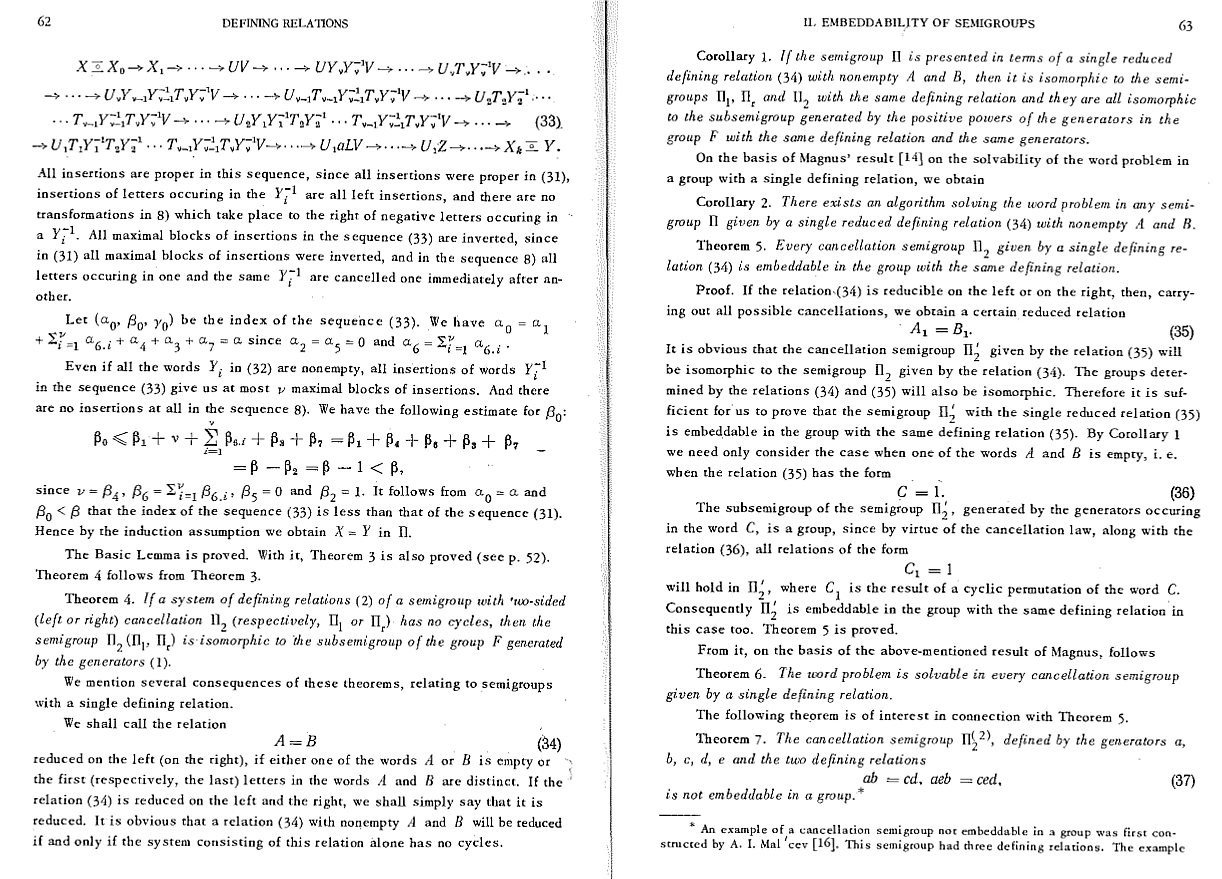
\includegraphics[height=0.65\textheight]{adjan.png}
	\end{center}

	\pause
	\vspace{-0.5cm}
	$\sim$60 pages of cases.
\end{frame}

\begin{frame}{One-relation special monoids}
	Zhang (1992) reproved the same result in 3 pages using rewriting systems. In both cases, the word problem for the semigroup is reduced to the word problem for the semigroup's group of units:\pskip

	\pause
	The \textbf{group of units} of a semigroup $S$ is the subgroup of $S$ consisting of all the invertible elements.
\end{frame}

\begin{frame}{One-relation special monoids}
	\begin{block}{Theorem (Zhang)}
		In a monoid $M$ with a presentation of the form
			\[ \Mon \langle a_1, \ldots, a_m \mid w_1 = \epsilon, \ldots, w_n = \epsilon \rangle, \]
		there is a presentation for the group of units with $n$ relations.
	\end{block}

	\pause
	\begin{block}{Corollary}
		If $M$ is a one-relator special monoid, the word problem for the group of units is solvable.
	\end{block}

	This follows from the above theorem and Magnus' result.
\end{frame}


\begin{frame}{Inverse monoids}
	A monoid in which element has an `inverse', in a slightly weaker sense than in a group.

	\pause
	\begin{block}{Theorem (Ivanov, Margolis, Meakin; 2001)}
		If the word problem is solvable for every inverse monoid admitting a presentation
			\[ \Inv \langle a_1, \ldots, a_m \mid w = \epsilon \rangle, \]
		then it is solvable for every one-relation semigroup.
	\end{block}
\end{frame}

\begin{frame}{A connection?}
	In their 2001 paper, Ivanov, Margolis and Meakin find a generating set for the group of units of the special inverse monoid.\pskip
	
	It is effectively the same as the generating set Zhang constructs for the group of units of a one-relation special monoid.\pskip

	But Zhang gives a whole presentation. Can we use a similar approach to find the needed relations in the inverse monoid case?
\end{frame}

\end{document}
